\documentclass[11pt,a4paper]{article}

\usepackage[T1]{fontenc}
\usepackage[utf8]{inputenc}
\usepackage{lmodern}
\usepackage{microtype}
\usepackage[a4paper,top=2.25cm,bottom=2.25cm,left=2.35cm,right=2.35cm]{geometry}
\usepackage[table]{xcolor}
\usepackage{graphicx}
\usepackage{booktabs}
\usepackage{tabularx}
\usepackage{array}
\usepackage{enumitem}
\usepackage{fancyhdr}
\usepackage{titlesec}
\usepackage{caption}
\usepackage{float}
\usepackage{listings}
\usepackage{amssymb}
\usepackage{hyperref}
\usepackage{lastpage}

% -----------------------------------------------------------------------------
% Replace these three values before submission.
% -----------------------------------------------------------------------------
\newcommand{\studentname}{Rakibul Hasan}
\newcommand{\studentid}{REPLACE\_STUDENT\_ID}
\newcommand{\studentsection}{REPLACE\_SECTION}
\newcommand{\githuburl}{https://github.com/USERNAME/cse472-web-lab-STUDENTID}
\newcommand{\submissiondate}{08 September 2026}

\definecolor{navy}{HTML}{102A43}
\definecolor{blue}{HTML}{1D4ED8}
\definecolor{cyan}{HTML}{0E8F93}
\definecolor{ink}{HTML}{243B53}
\definecolor{muted}{HTML}{627D98}
\definecolor{line}{HTML}{D9E2EC}
\definecolor{softblue}{HTML}{EDF4FF}
\definecolor{softcyan}{HTML}{EAFBFB}
\definecolor{success}{HTML}{087F5B}
\definecolor{softgreen}{HTML}{ECFDF5}
\definecolor{warning}{HTML}{A13D00}
\definecolor{warningbg}{HTML}{FFF1E7}
\definecolor{codebg}{HTML}{F4F7FA}

\hypersetup{
    colorlinks=true,
    linkcolor=blue,
    urlcolor=cyan,
    citecolor=blue,
    pdftitle={Lab Report 03: JavaScript Foundations and Simple Interaction},
    pdfauthor={Rakibul Hasan},
    pdfsubject={CSE472 Web and Internet Programming Lab}
}

\pagestyle{fancy}
\fancyhf{}
\fancyhead[L]{\small\color{muted}CSE472 \textbar{} Lab Report 03}
\fancyhead[R]{\small\color{muted}\studentid}
\fancyfoot[L]{\small\color{muted}Southeast University}
\fancyfoot[R]{\small\color{muted}Page \thepage\ of \pageref{LastPage}}
\renewcommand{\headrulewidth}{0.4pt}
\renewcommand{\footrulewidth}{0pt}

\titleformat{\section}
  {\Large\bfseries\color{navy}}
  {\thesection.}{0.65em}{}
  [\vspace{0.15em}{\color{line}\titlerule}]
\titleformat{\subsection}
  {\large\bfseries\color{navy}}
  {\thesubsection}{0.6em}{}
\titlespacing*{\section}{0pt}{1.2em}{0.75em}
\titlespacing*{\subsection}{0pt}{1em}{0.45em}

\setlist[itemize]{leftmargin=1.55em,itemsep=0.35em,topsep=0.35em}
\setlist[enumerate]{leftmargin=1.75em,itemsep=0.45em,topsep=0.35em}
\setlength{\parindent}{0pt}
\setlength{\parskip}{0.62em}
\renewcommand{\arraystretch}{1.28}
\captionsetup{font=small,labelfont={bf,color=navy},textfont={color=ink}}

\newcolumntype{Y}{>{\raggedright\arraybackslash}X}
\newcolumntype{L}[1]{>{\raggedright\arraybackslash}p{#1}}
\setlength{\emergencystretch}{2em}

\lstdefinelanguage{JavaScript}{
    keywords={break,case,catch,const,continue,default,delete,do,else,false,finally,
      for,function,if,in,let,new,null,return,switch,true,try,typeof,var,while},
    sensitive=true,
    morecomment=[l]{//},
    morecomment=[s]{/*}{*/},
    morestring=[b]",
    morestring=[b]'
}

\lstdefinestyle{labcode}{
    language=JavaScript,
    backgroundcolor=\color{codebg},
    basicstyle=\ttfamily\small,
    keywordstyle=\color{blue}\bfseries,
    stringstyle=\color{success},
    commentstyle=\color{cyan},
    numbers=left,
    numberstyle=\scriptsize\color{muted},
    numbersep=9pt,
    frame=single,
    rulecolor=\color{line},
    breaklines=true,
    showstringspaces=false,
    tabsize=4,
    xleftmargin=0.3em,
    framexleftmargin=0.3em
}

\newcommand{\statuspass}{\textcolor{success}{\textbf{PASS}}}
\newcommand{\placeholder}[1]{\colorbox{warningbg}{\textcolor{warning}{\strut\texttt{#1}}}}

\begin{document}
\pagenumbering{roman}

% =============================================================================
% 1. Cover page
% =============================================================================
\begin{titlepage}
    \thispagestyle{empty}
    {\color{navy}\rule{\textwidth}{7pt}}

    \vspace{1.1cm}
    {\large\bfseries\color{cyan}SOUTHEAST UNIVERSITY}\par
    \vspace{0.15cm}
    {\large\color{ink}Department of Computer Science and Engineering}\par

    \vspace{1.35cm}
    {\small\bfseries\color{muted}\MakeUppercase{CSE472: Web and Internet Programming Lab}}\par
    \vspace{0.45cm}
    {\fontsize{31}{37}\selectfont\bfseries\color{navy}Lab Report 03}\par
    \vspace{0.28cm}
    {\fontsize{22}{28}\selectfont\bfseries\color{blue}JavaScript Foundations and\\Simple Interaction}\par

    \vspace{0.7cm}
    \colorbox{softcyan}{%
        \begin{minipage}{0.94\textwidth}
            \vspace{0.32cm}
            \centering
            {\large\bfseries\color{navy}Student Workshop Registration System}\par
            \vspace{0.12cm}
            {\color{muted}Project Stage 03: Making the webpage interactive with JavaScript}
            \vspace{0.32cm}
        \end{minipage}
    }

    \vfill

    \begin{tabularx}{\textwidth}{L{0.34\textwidth}Y}
        \toprule
        \rowcolor{softblue}
        \textbf{Student information} & \textbf{Details} \\
        \midrule
        Student name & \studentname \\
        Student ID & \placeholder{\studentid} \\
        Section & \placeholder{\studentsection} \\
        Department & Computer Science and Engineering \\
        Submission date & \submissiondate \\
        GitHub repository & \href{\githuburl}{\texttt{github.com/USERNAME/cse472-web-lab-STUDENTID}} \\
        Lab 03 folder & \texttt{labs/lab-03-javascript/} \\
        \bottomrule
    \end{tabularx}

    \vspace{0.65cm}
    \colorbox{warningbg}{%
        \begin{minipage}{0.94\textwidth}
            \vspace{0.22cm}
            \textcolor{warning}{\textbf{Before submission:}} Replace the highlighted Student ID and Section, then replace the GitHub URL with the actual repository link.
            \vspace{0.22cm}
        \end{minipage}
    }

    \vfill
    {\color{line}\rule{\textwidth}{0.8pt}}\par
    {\small\color{muted}Prepared for academic submission in CSE472}
\end{titlepage}

\pagenumbering{arabic}
\setcounter{section}{1}

% =============================================================================
% 2. Objectives
% =============================================================================
\section{Objectives}

The purpose of this laboratory was to extend the Student Workshop Registration System from a static HTML and CSS page into an interactive webpage. The specific objectives were to:

\begin{itemize}
    \item connect an external JavaScript file to the existing webpage;
    \item use a variable to store the number of available workshop seats;
    \item apply a basic \texttt{if...else} condition to select the correct seat message;
    \item create functions and call them from HTML buttons using \texttt{onclick};
    \item select elements with \texttt{document.getElementById()}, read an input with \texttt{.value}, and update page text with \texttt{.textContent}; and
    \item implement and test one small independent improvement while keeping the code within the concepts introduced in Lab 03.
\end{itemize}

% =============================================================================
% 3. Tools used
% =============================================================================
\section{Tools Used}

\begin{table}[H]
    \centering
    \caption{Tools used to implement and verify Lab 03}
    \begin{tabularx}{\textwidth}{L{0.30\textwidth}Y}
        \toprule
        \rowcolor{navy}
        \textcolor{white}{\textbf{Tool}} & \textcolor{white}{\textbf{Purpose}} \\
        \midrule
        Visual Studio Code & Created and edited \texttt{index.html}, \texttt{css/style.css}, and \texttt{js/script.js}. \\
        Modern web browser & Opened the page, activated buttons, entered a name, and observed text changes. \\
        Browser Developer Tools & Checked element IDs, function connections, and JavaScript errors during debugging. \\
        Node.js & Performed repeatable JavaScript interaction checks against controlled page elements. \\
        Git and GitHub & Versioned the work and stored it in the required course repository structure. \\
        LaTeX & Prepared the report with structured sections, figures, tables, links, and captions. \\
        \bottomrule
    \end{tabularx}
\end{table}

% =============================================================================
% 4. Work completed
% =============================================================================
\section{Work Completed}

The Lab 02 layout was retained as a responsive registration webpage, while all required behaviour was placed in the new external file \texttt{js/script.js}. Figure~\ref{fig:overview} shows the completed workshop page structure.

\begin{figure}[H]
    \centering
    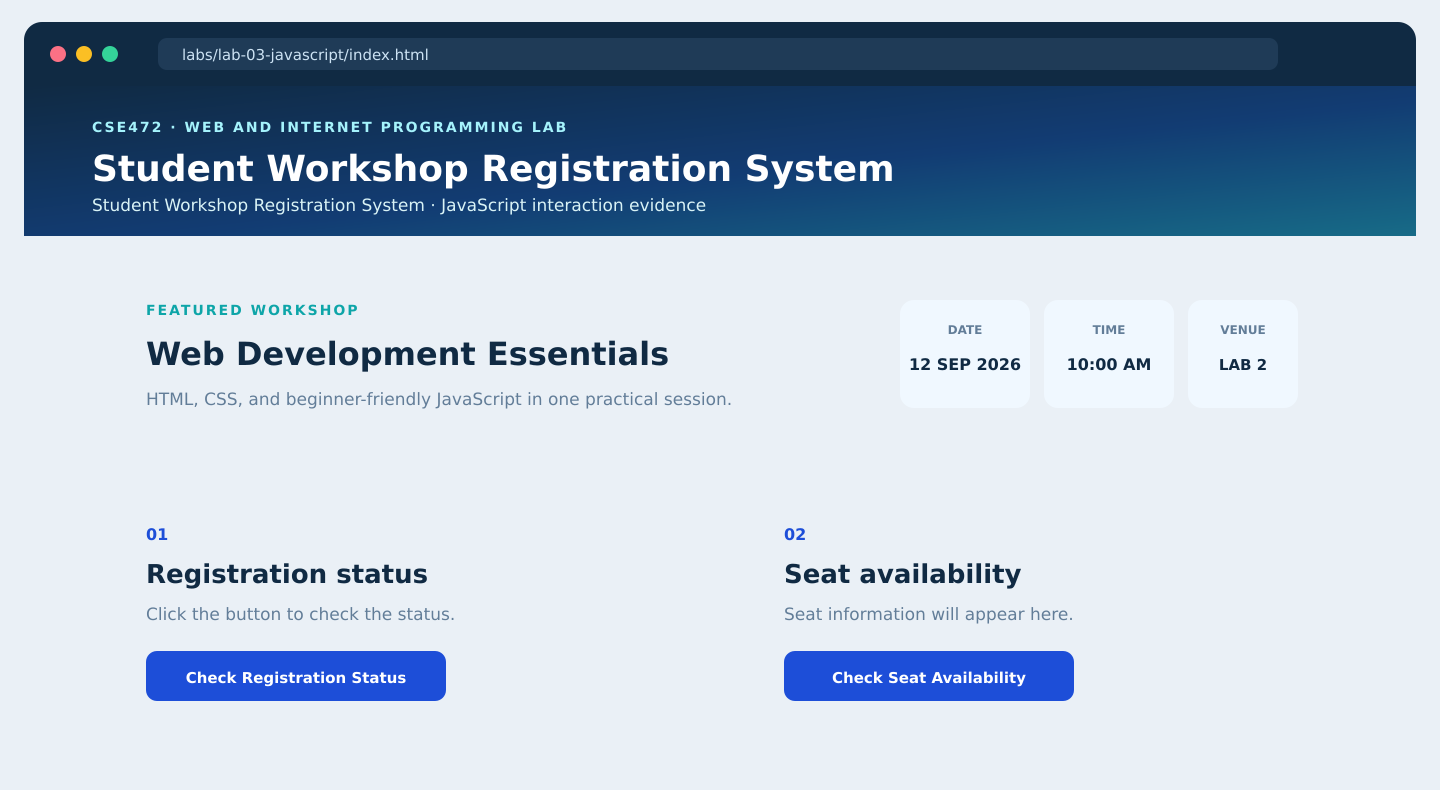
\includegraphics[width=0.96\textwidth]{figures/output_overview.png}
    \caption{Completed Student Workshop Registration System interface.}
    \label{fig:overview}
\end{figure}

\subsection*{Registration status interaction}
The \textit{Check Registration Status} button calls \texttt{checkRegistration()}. The function selects \texttt{registrationStatus} and replaces its original instruction with ``Registration is currently open.''

\subsection*{Seat availability interaction}
The variable \texttt{availableSeats} initially stores \texttt{12}. The \texttt{checkSeats()} function uses \texttt{if...else}: a positive value displays the remaining seat count, while zero displays the full-workshop message.

\subsection*{Personal greeting interaction}
The \texttt{showGreeting()} function reads the current value of \texttt{studentName}. It joins the typed name with a welcome message and writes the result into \texttt{greetingMessage}.

\subsection*{Independent improvement}
A \textit{Show Venue} button was added as the independent improvement. It calls \texttt{showVenue()} and changes the \texttt{venueMessage} paragraph to a short venue reminder. This feature uses only a function, \texttt{onclick}, \texttt{getElementById()}, and \texttt{textContent}.

% =============================================================================
% 5. Implementation evidence
% =============================================================================
\section{Implementation Evidence}

The selected evidence below focuses on the required connections and visible interaction results. The code images come directly from the submitted source files, and the output states were compared against the executed JavaScript tests.

\begin{figure}[H]
    \centering
    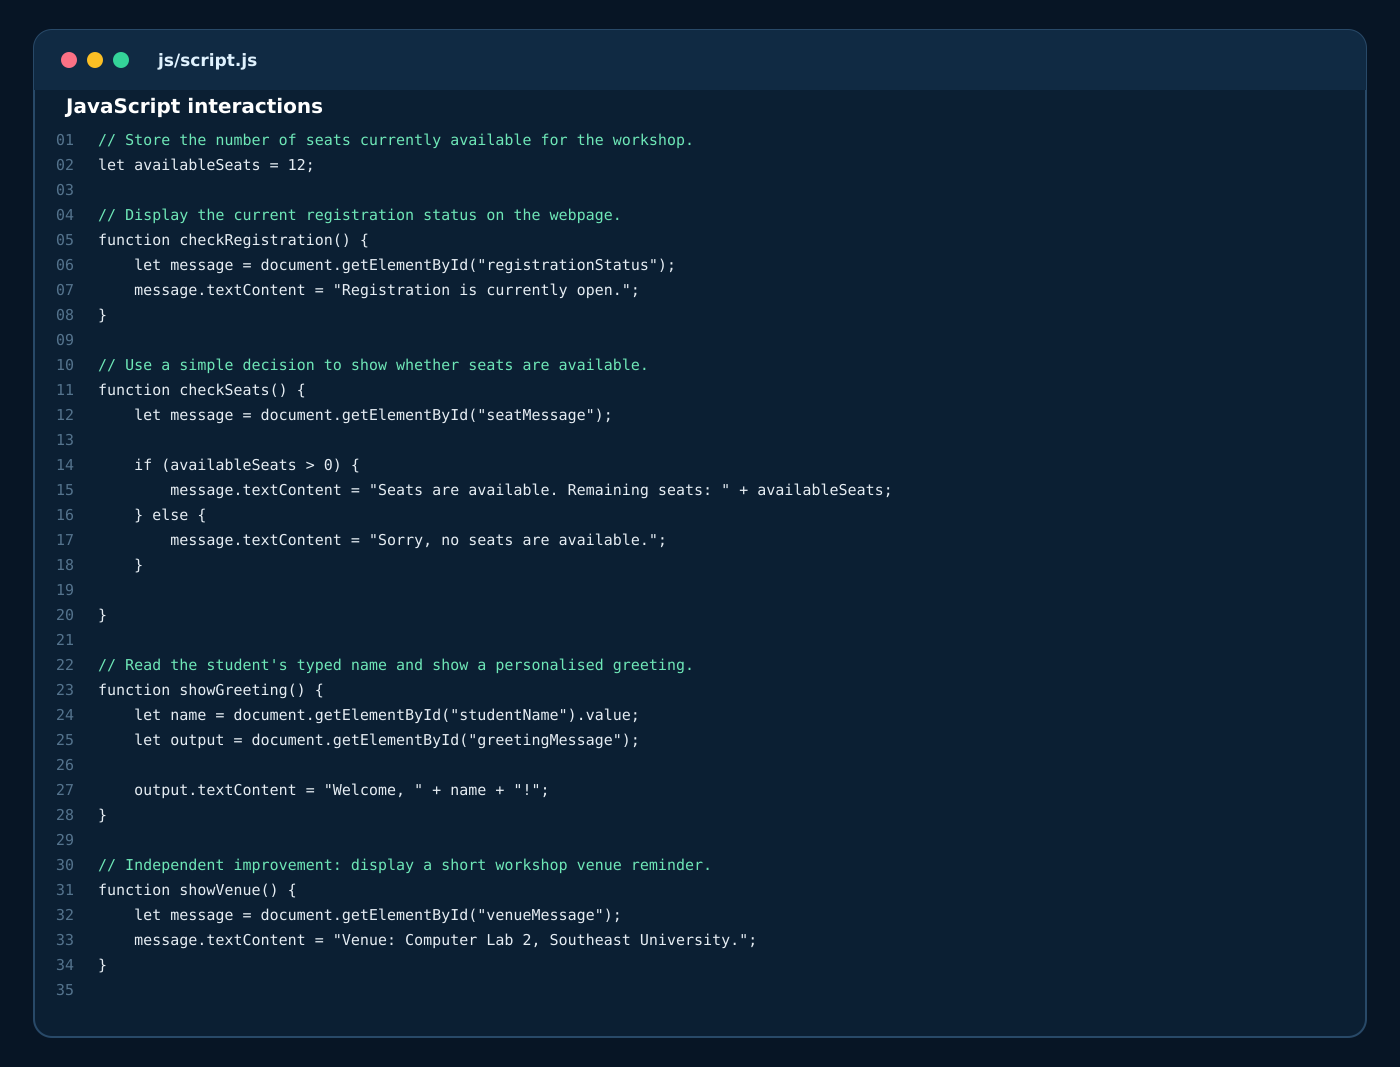
\includegraphics[width=0.92\textwidth,height=0.72\textheight,keepaspectratio]{figures/code_javascript.png}
    \caption{Important sections of the completed external JavaScript file.}
    \label{fig:javascript-code}
\end{figure}

\begin{figure}[H]
    \centering
    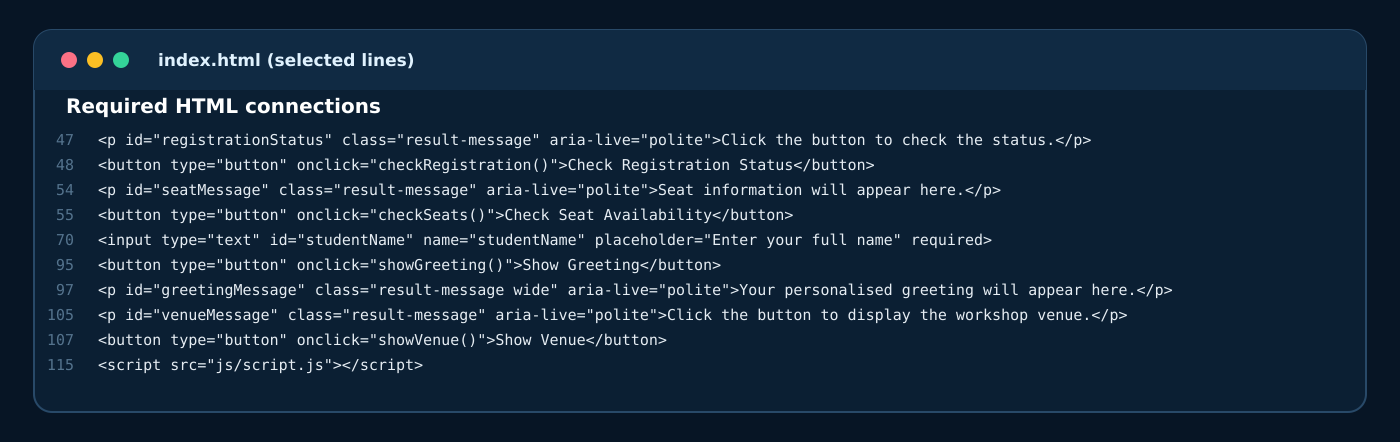
\includegraphics[width=0.96\textwidth]{figures/code_html_connections.png}
    \caption{Selected HTML IDs, \texttt{onclick} calls, and external script connection.}
    \label{fig:html-connections}
\end{figure}

\begin{figure}[H]
    \centering
    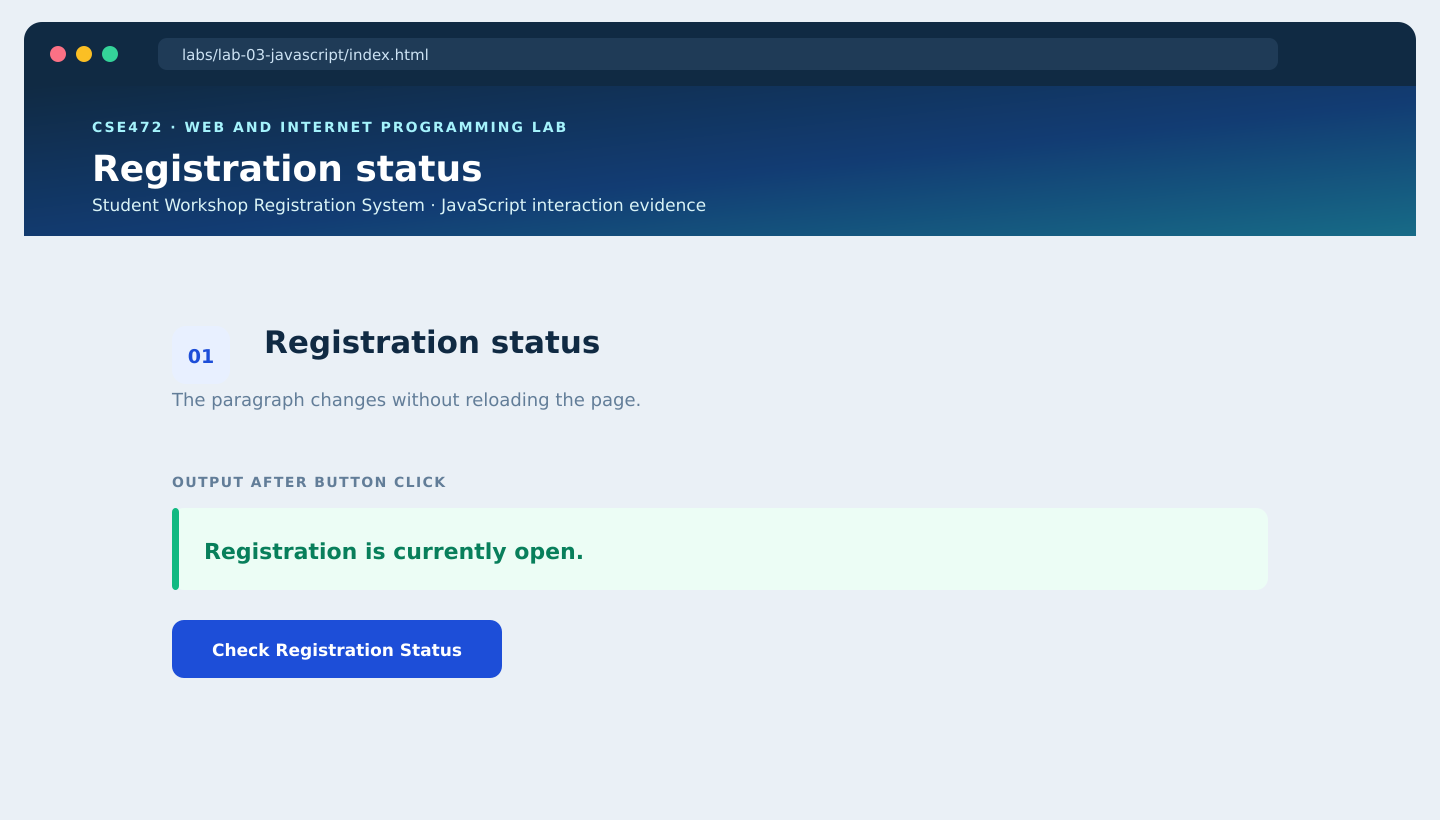
\includegraphics[width=0.94\textwidth]{figures/output_registration.png}
    \caption{Output after clicking \textit{Check Registration Status}.}
    \label{fig:registration-output}
\end{figure}

\begin{figure}[H]
    \centering
    \begin{minipage}[t]{0.49\textwidth}
        \centering
        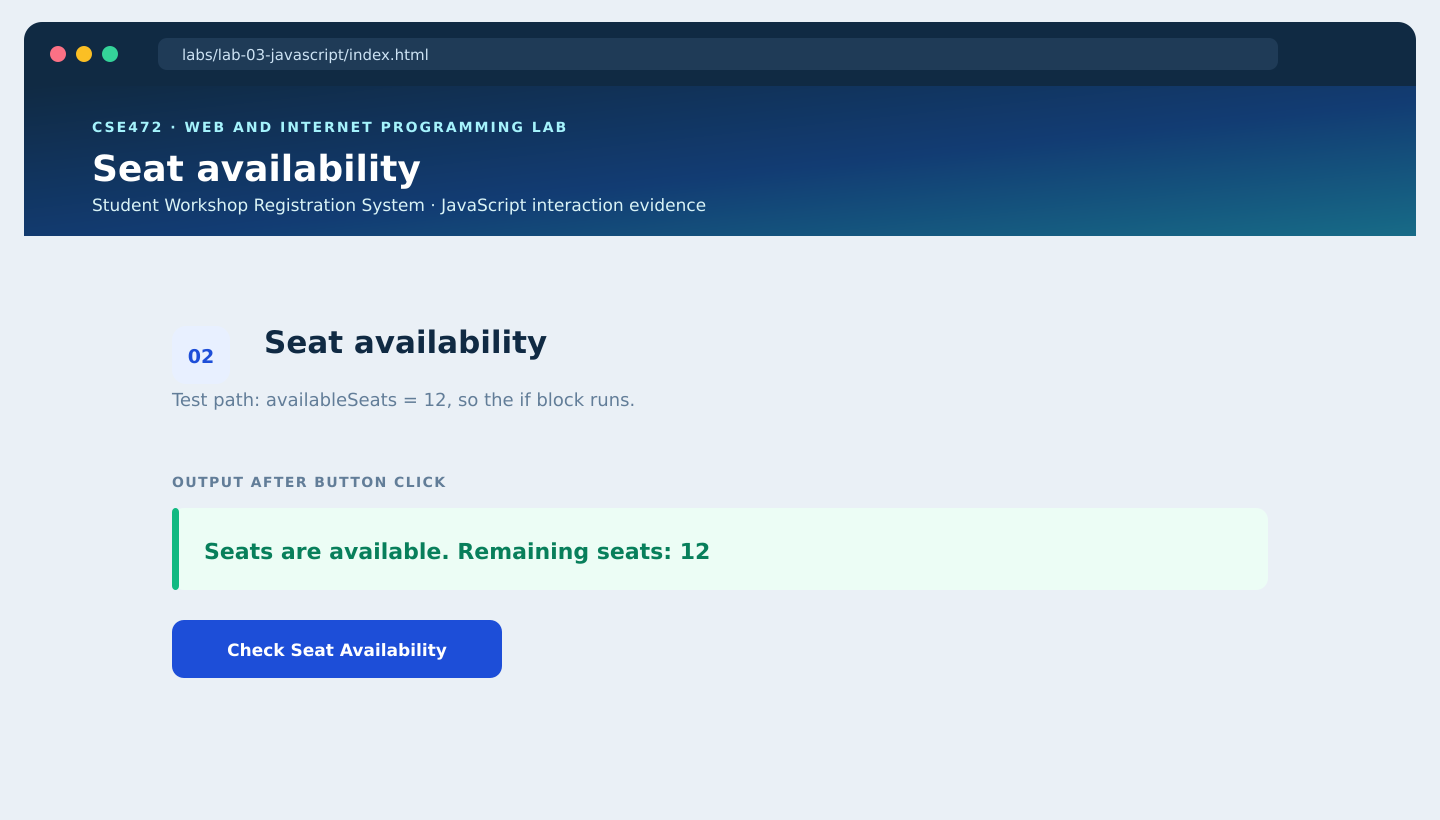
\includegraphics[width=\textwidth]{figures/output_seats_available.png}
        \captionof{figure}{Seat checker with \texttt{availableSeats = 12}.}
        \label{fig:seats-open}
    \end{minipage}\hfill
    \begin{minipage}[t]{0.49\textwidth}
        \centering
        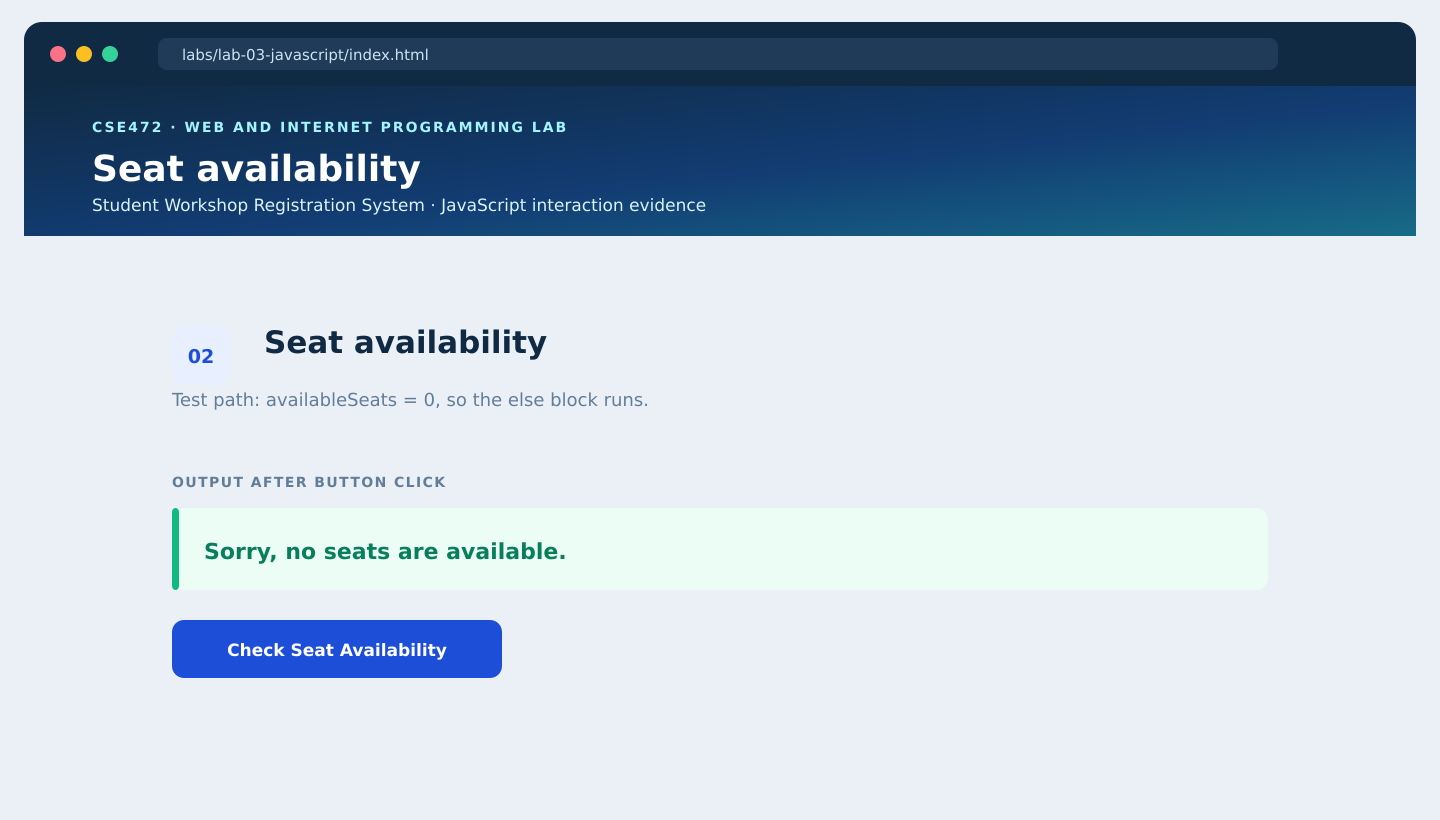
\includegraphics[width=\textwidth]{figures/output_seats_full.png}
        \captionof{figure}{Seat checker with \texttt{availableSeats = 0}.}
        \label{fig:seats-full}
    \end{minipage}
\end{figure}

Figures~\ref{fig:seats-open} and~\ref{fig:seats-full} demonstrate both branches of the required condition. The original value was restored to \texttt{12} after the zero-seat test.

\begin{figure}[H]
    \centering
    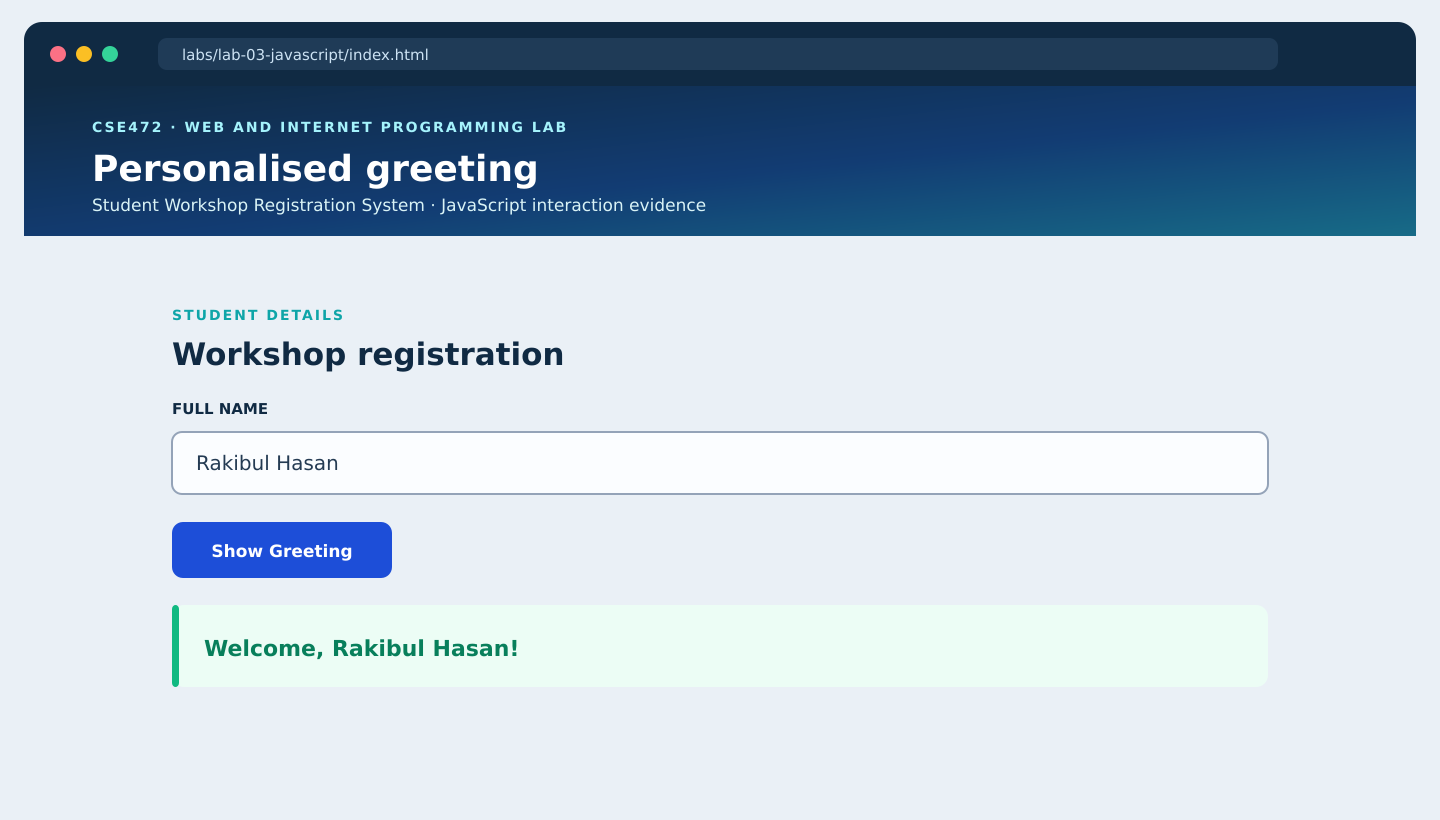
\includegraphics[width=0.94\textwidth]{figures/output_greeting.png}
    \caption{Personalised greeting after reading ``Rakibul Hasan'' from the Full Name input.}
    \label{fig:greeting-output}
\end{figure}

\begin{figure}[H]
    \centering
    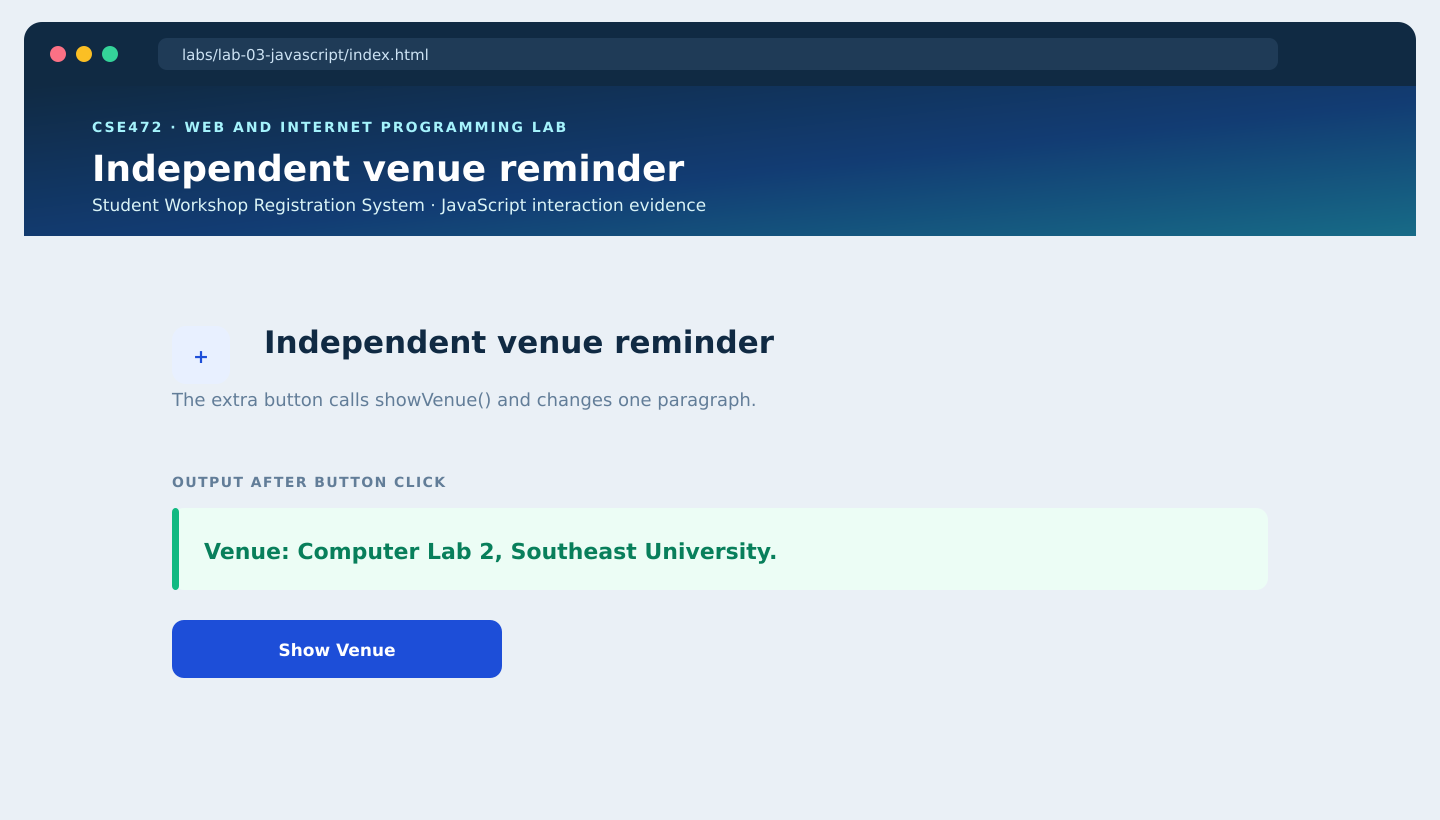
\includegraphics[width=0.94\textwidth]{figures/output_venue.png}
    \caption{Independent venue-reminder interaction.}
    \label{fig:venue-output}
\end{figure}

% =============================================================================
% 6. Key JavaScript explanation
% =============================================================================
\clearpage
\section{Key JavaScript Explanation}

\begin{table}[H]
    \centering
    \small
    \caption{Lab 03 JavaScript concepts explained using the implemented code}
    \begin{tabularx}{\textwidth}{L{0.19\textwidth}L{0.34\textwidth}Y}
        \toprule
        \rowcolor{navy}
        \textcolor{white}{\textbf{Concept}} & \textcolor{white}{\textbf{Example}} & \textcolor{white}{\textbf{Explanation}} \\
        \midrule
        Variable & \texttt{let availableSeats = 12;} & Stores a value under a meaningful name so it can be used later. \\
        \rowcolor{softblue}
        \texttt{if...else} & \texttt{if (availableSeats > 0)} & Chooses between the available-seat message and the no-seat message. \\
        Function & \texttt{function checkSeats() \{...\}} & Groups related instructions under a name. Creating it defines the instructions; calling it runs them. \\
        \rowcolor{softblue}
        \texttt{onclick} & \texttt{onclick="checkSeats()"} & Calls the named JavaScript function when the user clicks the HTML button. \\
        \texttt{getElementById()} & \texttt{getElementById("seatMessage")} & Finds the unique HTML element whose \texttt{id} is exactly \texttt{seatMessage}. The letter case must match. \\
        \rowcolor{softblue}
        \texttt{textContent} & \texttt{message.textContent = ...} & Replaces the visible text inside the selected paragraph. \\
        \texttt{value} & \texttt{getElementById("studentName")}\\\texttt{.value} & Reads the text currently typed into the Full Name input. \\
        \bottomrule
    \end{tabularx}
\end{table}

For example, clicking the seat button calls \texttt{checkSeats()}. The function finds the \texttt{seatMessage} paragraph, checks \texttt{availableSeats}, and changes the paragraph's \texttt{textContent}. The page does not need to reload.

% =============================================================================
% 7. Testing and corrections
% =============================================================================
\section{Testing and Corrections}

Each required interaction was tested separately. A repeatable JavaScript check also confirmed that the expected HTML connections were present and that every function named by \texttt{onclick} existed. All seven automated checks passed.

\begin{table}[H]
    \centering
    \footnotesize
    \caption{Functional testing results}
    \begin{tabularx}{\textwidth}{L{0.26\textwidth}L{0.23\textwidth}Y L{0.09\textwidth}}
        \toprule
        \rowcolor{navy}
        \textcolor{white}{\textbf{Test}} & \textcolor{white}{\textbf{Input or action}} & \textcolor{white}{\textbf{Expected and observed result}} & \textcolor{white}{\textbf{Status}} \\
        \midrule
        Script connection & Load \texttt{index.html} & External file path is \texttt{js/script.js}; all functions execute. & \statuspass \\
        \rowcolor{softblue}
        Registration status & Click status button & Paragraph becomes ``Registration is currently open.'' & \statuspass \\
        Seat availability, true path & Set seats to 12; click button & Remaining-seat message displays 12. & \statuspass \\
        \rowcolor{softblue}
        Seat availability, false path & Set seats to 0; click button & ``Sorry, no seats are available.'' is displayed. & \statuspass \\
        Personal greeting & Enter ``Rakibul Hasan''; click greeting & ``Welcome, Rakibul Hasan!'' is displayed. & \statuspass \\
        \rowcolor{softblue}
        Independent improvement & Click \textit{Show Venue} & Computer Lab 2 venue reminder appears. & \statuspass \\
        Function-name check & Inspect every \texttt{onclick} call & No missing or incorrectly cased function names. & \statuspass \\
        \bottomrule
    \end{tabularx}
\end{table}

\subsection*{Error identified and corrected}
The required debugging check showed why exact letter case matters. A deliberately mismatched lookup such as \texttt{registrationstatus} does not find the HTML element named \texttt{registrationStatus}. The lookup was corrected so the HTML \texttt{id} and the argument passed to \texttt{getElementById()} match exactly. The same case check was applied to every function name used by \texttt{onclick}.

The detailed machine-readable result is included in the submission package as \path{evidence/automated_test_results.txt}.

% =============================================================================
% 8. GitHub link
% =============================================================================
\section{GitHub Link}

The source code is organised in the required repository location:

\begin{center}
    \fcolorbox{line}{softblue}{%
        \begin{minipage}{0.86\textwidth}
            \vspace{0.18cm}
            \textbf{Repository:} \href{\githuburl}{\texttt{\githuburl}}\\[0.18cm]
            \textbf{Required folder:} \texttt{labs/lab-03-javascript/}
            \vspace{0.18cm}
        \end{minipage}
    }
\end{center}

\textcolor{warning}{\textbf{Final edit required:}} Replace the placeholder URL above with the actual personal GitHub repository link before submitting the PDF.

The suggested commit message is: \texttt{Complete Lab 03 JavaScript interactions}.

% =============================================================================
% 9. Learning reflection
% =============================================================================
\section{Learning Reflection}

\begin{enumerate}
    \item \textbf{What is one clear difference between HTML and JavaScript?}\\
    HTML defines the structure and content of the webpage, such as headings, inputs, paragraphs, and buttons. JavaScript adds behaviour, such as responding to a click, reading typed information, making a decision, and changing visible text.

    \item \textbf{Which JavaScript concept was most useful in this laboratory? Why?}\\
    The combination of functions and \texttt{getElementById()} was most useful. A function keeps each interaction organised, while \texttt{getElementById()} connects that function to a specific part of the webpage. Together they make the button actions clear and reusable.

    \item \textbf{Describe one error you faced and how you fixed it.}\\
    A case mismatch between \texttt{registrationstatus} and \texttt{registrationStatus} prevented the intended element from being found during the debugging check. I fixed it by matching the JavaScript lookup exactly to the HTML \texttt{id}, then checked all remaining IDs and function names in the same way.

    \item \textbf{What simple JavaScript improvement did you add independently?}\\
    I added a \textit{Show Venue} button. When clicked, it calls \texttt{showVenue()}, finds the \texttt{venueMessage} paragraph, and updates the paragraph with the workshop venue.
\end{enumerate}

% =============================================================================
% 10. AI assistance declaration
% =============================================================================
\clearpage
\section{AI Assistance Declaration}

\fcolorbox{cyan}{softcyan}{%
    \begin{minipage}{0.92\textwidth}
        \vspace{0.28cm}
        I used \textbf{ChatGPT} to help organise the report, check the JavaScript logic, generate repeatable test evidence, and improve the clarity of the written explanations. I checked the generated code by reviewing each function, confirming the HTML IDs and \texttt{onclick} names, running both paths of the seat condition, comparing every output with its expected text, and keeping the implementation within the concepts taught in Lab 03.
        \vspace{0.28cm}
    \end{minipage}
}

\clearpage
\appendix

% =============================================================================
% Appendix A
% =============================================================================
\section{Practice Set Answers}

\subsection*{Predict the result}
\begin{enumerate}
    \item The value of \texttt{remaining} is \texttt{5}, because \texttt{8 - 3 = 5}.
    \item The browser displays \texttt{Full}, because \texttt{availableSeats} is zero and the condition \texttt{availableSeats > 0} is false.
\end{enumerate}

\subsection*{Small coding tasks}

\begin{lstlisting}[style=labcode,caption={Practice variables and functions}]
let courseName = "CSE472";
alert(courseName);

function showCourse() {
    alert("Web and Internet Programming Lab");
}

function showNotice() {
    let notice = document.getElementById("notice");
    notice.textContent = "Lab starts at 9:00 AM.";
}

function showStudentId() {
    let id = document.getElementById("studentId").value;
    let output = document.getElementById("idOutput");
    output.textContent = "Student ID: " + id;
}
\end{lstlisting}

\begin{lstlisting}[style=labcode,language=HTML,caption={Practice HTML connections}]
<button type="button" onclick="showCourse()">Show Course</button>

<p id="notice">Waiting for the lab notice.</p>
<button type="button" onclick="showNotice()">Show Notice</button>

<input type="text" id="studentId">
<button type="button" onclick="showStudentId()">Show Student ID</button>
<p id="idOutput"></p>
\end{lstlisting}

\subsection*{Concept explanations}
\begin{itemize}
    \item JavaScript adds behaviour and interaction to a webpage.
    \item An HTML \texttt{id} must match \texttt{getElementById()} exactly so the browser can find the intended element.
    \item Creating a function defines its instructions; calling the function with parentheses runs those instructions.
    \item \texttt{.value} reads the current content of an input field.
    \item \texttt{.textContent} reads or changes the text inside an HTML element.
\end{itemize}

% =============================================================================
% Appendix B
% =============================================================================
\section{Project Structure and Submission Checklist}

\subsection*{Required project structure}
\begin{lstlisting}[style=labcode,language={}]
labs/
`-- lab-03-javascript/
    |-- index.html
    |-- css/
    |   `-- style.css
    |-- js/
    |   `-- script.js
    `-- assets/
        `-- images/
\end{lstlisting}

\subsection*{Final checks}
\begin{tabularx}{\textwidth}{L{0.08\textwidth}Y}
    \toprule
    \rowcolor{navy}
    \textcolor{white}{\textbf{Done}} & \textcolor{white}{\textbf{Checklist item}} \\
    \midrule
    \textcolor{success}{$\boxtimes$} & The report has the correct Lab 03 title and all ten required sections. \\
    \rowcolor{softblue}
    \textcolor{success}{$\boxtimes$} & The code uses the required external JavaScript file and exact project folder. \\
    \textcolor{success}{$\boxtimes$} & Selected code and interaction evidence include captions. \\
    \rowcolor{softblue}
    \textcolor{success}{$\boxtimes$} & Registration status, both seat paths, greeting, and independent button were tested. \\
    \textcolor{success}{$\boxtimes$} & Reflection answers and the AI assistance declaration are included. \\
    \rowcolor{warningbg}
    \textcolor{warning}{$\square$} & Replace Student ID, Section, and GitHub URL; then rename the PDF to \texttt{CSE472\_Lab03\_StudentID.pdf}. \\
    \bottomrule
\end{tabularx}

\vfill
\begin{center}
    \color{muted}\small End of Lab Report 03
\end{center}

\end{document}
